% Send to Mandar,Jayesh,Arnab,Deepak and perhaps Rahee
\documentclass{article}
\newcommand{\beq}{\begin{equation}}
\newcommand{\eeq}{\end{equation}}
\newcommand{\ber}{\begin{eqnarray}}
\newcommand{\eer}{\end{eqnarray}}
\newcommand{\nn}{\nonumber}
\newcommand{\dd}[2]{\frac{d}{d{#2}}{(#1)} }
\newcommand{\pdd}[2]{\frac{\partial}{\partial{#2}}{(#1)} }
\usepackage{amsmath}
\usepackage{amsfonts}
\usepackage{url}
\usepackage{graphicx}
\usepackage{caption}
\usepackage{subcaption}
\usepackage{multirow}
\begin{document}
\title{Circle identification using Convolutional Neural Networks in TensorFlow}
\author{Nachiket Gokhale}
\date{\today}
\maketitle
\section{Introduction}
We consider a dataset consisting of images of stiffness of the type shown in Figure (\ref{fig:sampleimages}). All images are 64 pixels by 64 pixels. Unlike standard RGB images which have three channels, these images have only one channel. So, the shape of each image is $(64,64,1)$. The value of the background stiffness is $1$ and the value of the circle stiffness is a real number which ranges from $2.0$ to $5.0$. Each image contains only one circle or is homogeneous (no circles). We consider the following problems
\begin{enumerate}
\item{\textbf{Binary classification}: Given a stiffness image classify it into homogneous (label 0)or having an inclusion (label 1)}
\item{\textbf{Predicting stiffness location:} Given a stiffness image containing a circle find the center of the circle}
\item{\textbf{Predicting stiffness value:} Given a stiffness image containing a circle find the value of the stiffness of the circle}
\item{\textbf{Predicting circle radius:} Given a stiffness image containing a circle find the radius of the circle}
\end{enumerate}
\begin{figure}
  \centering
  \begin{subfigure}[b]{0.45\textwidth}
    \centering
    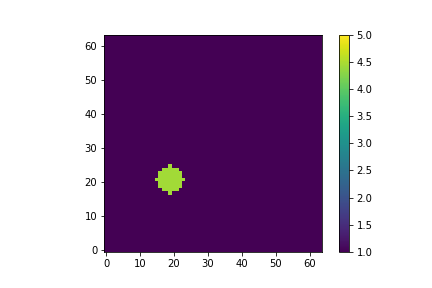
\includegraphics[totalheight=4cm]{circle_id/sample0.png}
    \caption{Sample image 1}
  \end{subfigure}
  %
  \begin{subfigure}[b]{0.45\textwidth}
    \centering
    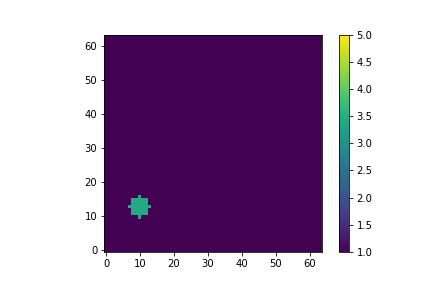
\includegraphics[totalheight=4cm]{circle_id/sample1.png}
    \caption{Sample image 2}
  \end{subfigure}
  %
  \begin{subfigure}[b]{0.45\textwidth}
    \centering
    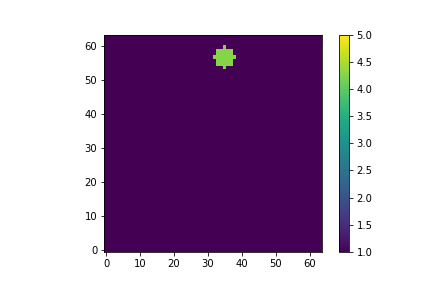
\includegraphics[totalheight=4cm]{circle_id/sample2.png}
    \caption{Sample image 3}
  \end{subfigure}
  \begin{subfigure}[b]{0.45\textwidth}
    \centering
    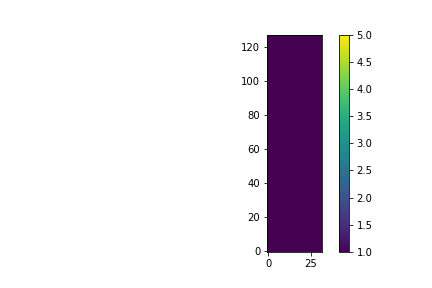
\includegraphics[totalheight=4cm]{circle_id/sample3.png}
    \caption{Sample image 4}
  \end{subfigure}
  %
  \begin{subfigure}[b]{0.45\textwidth}
    \centering
    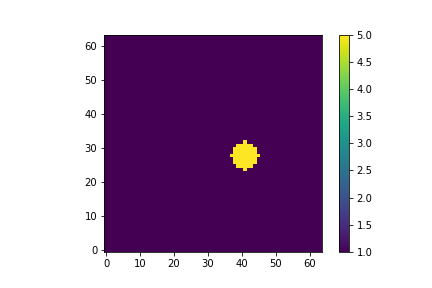
\includegraphics[totalheight=4cm]{circle_id/sample4.png}
    \caption{Sample image 5}
  \end{subfigure}
  %
  \begin{subfigure}[b]{0.45\textwidth}
    \centering
    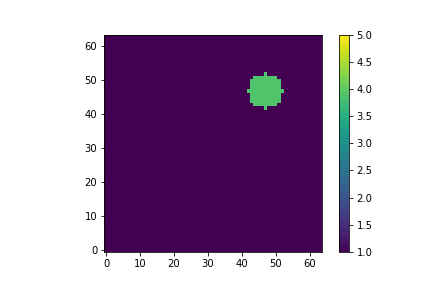
\includegraphics[totalheight=4cm]{circle_id/sample5.png}
    \caption{Sample image 6}
  \end{subfigure}
\caption{\label{fig:sampleimages} Sample images in the image dataset}
\end{figure}
%
\section{Binary classification}
We have $1024$ training images, $205$ validation images and $205$ test imagees. We set maximum epochs to $512$ and terminate the training process if the validation loss function does not change by more than $10^{-4}$ over $10$ epochs. We first feature scale the images using the standard deviation. The loss function is 'binary\_crossentropy'. There were $701$ positive (with circle) training examples and $323$ negative training examples. \\ The CNN is shown in Figure (\ref{fig:binary_model}). This architecture is the same as a CNN to classify images into two categories: 'cat' or 'dog'. The CNN has $812,641$ trainable parameters. Maybe this is overfitting the data. And the good results that are seen are a consequence of this. It is also observed that the training of the CNN is quite strongly dependent on the initial random choice of parameters. The metrics for binary classification are shown in Figure (\ref{fig:binarymetrics}). We get an accuracy score of $1.0$ right from the start. The confusion matrix is shown in Figure 
\begin{figure}
   \centering
    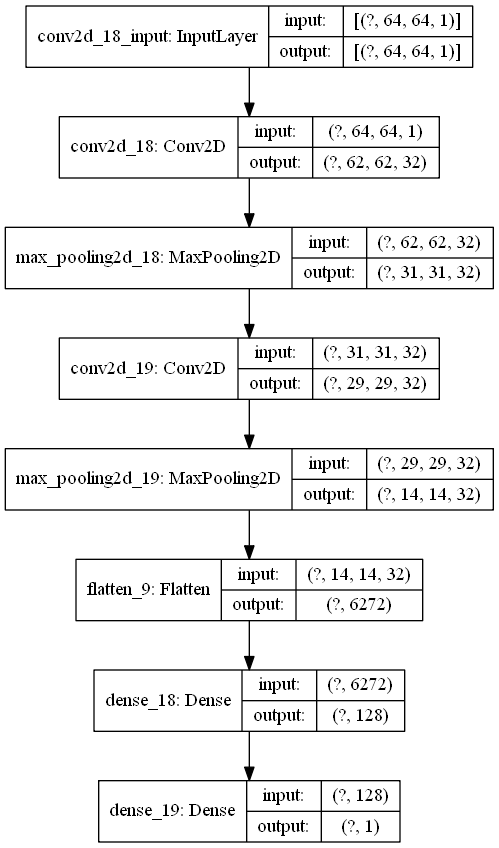
\includegraphics[totalheight=8cm]{circle_id/binary/model.png}
  \caption{\label{fig:binary_model} CNN for binary classification}
\end{figure}
%
\begin{figure}
\centering
\begin{subfigure}[b]{0.45\textwidth}
    \centering
    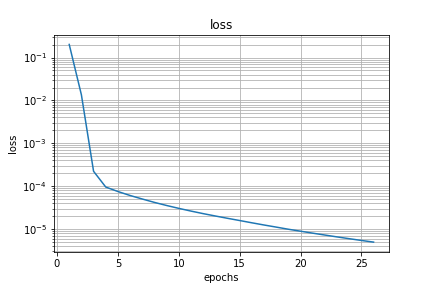
\includegraphics[totalheight=4cm]{circle_id/binary/plotloss.png}
    \caption{Training loss}
  \end{subfigure}
%
\begin{subfigure}[b]{0.45\textwidth}
    \centering
    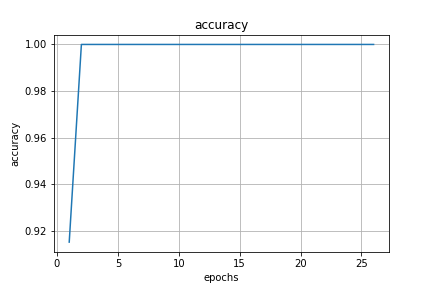
\includegraphics[totalheight=4cm]{circle_id/binary/plotaccuracy.png}
    \caption{Training accuracy}
  \end{subfigure}
%
\begin{subfigure}[b]{0.45\textwidth}
    \centering
    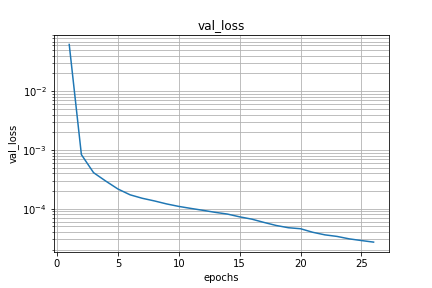
\includegraphics[totalheight=4cm]{circle_id/binary/plotval_loss.png}
    \caption{Validation loss}
  \end{subfigure}
%
\begin{subfigure}[b]{0.45\textwidth}
    \centering
    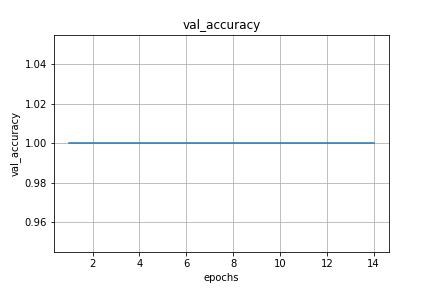
\includegraphics[totalheight=4cm]{circle_id/binary/plotval_accuracy.png}
    \caption{Validation accuracy}
  \end{subfigure}
\caption{\label{fig:binarymetrics} Metrics for binary classification}
\end{figure}
%
\begin{center}
  \begin{tabular}{cccc}
    \cline{3-4}
    & & \multicolumn{2}{|c|}{Actual class}  \\
    \cline{3-4}
    & & \multicolumn{1}{|c|}{Circle} &  \multicolumn{1}{|c|}{No Circle}\\
    \hline
    \multicolumn{1}{|c}{Predicted} & \multicolumn{1}{|c|}{Circle} & \multicolumn{1}{|c|}{47} & \multicolumn{1}{|c|}{0} \\
    \cline{2-4}
    \multicolumn{1}{|c}{class} & \multicolumn{1}{|c|}{no circle} & \multicolumn{1}{|c|}{0} & \multicolumn{1}{|c|}{158}\\
    \hline
  \end{tabular}
\end{center}
\section{Predicting stiffness location}
%
\section{Predicting stiffness value}
%
\section{Predicting circle radius}
%
\end{document}
